%%
%%       --- a chapter ---
%%
%% A chapter

\chapter[Data and Sample Selection]{Photmetric data and high-redshift sample selection} 
\label{ch:chapter1_label}

\section{The Data}\label{sec:data}
The photometry used throughout this work is taken from the catalog of \citet{Guo:2013ig}, a UV to mid-infrared multi-wavelength catalog in the CANDELS GOODS South field based on the CANDELS WFC3/IR observations combined with existing public data.

\subsection{Imaging Data}
The near-infrared WFC3/IR data combines observations from the CANDELS survey \citep{2011ApJS..197...35G,Koekemoer:2011br} with the WFC3 Early Release Science (ERS; \citeauthor{2011ApJS..193...27W}~\citeyear{2011ApJS..193...27W}) and Hubble Ultra Deep Field (HUDF; PI Illingworth; \citeauthor{Bouwens:2010dk}~\citeyear{Bouwens:2010dk}) surveys. The southern two thirds of the field (incorporating the CANDELS `DEEP' and `WIDE' regions and the UDF) were observed in the F105W, F125W and F160W bands. The northern-most third, comprising the ERS region, was observed in F098M, F125W and F160W. In addition to the initial CANDELS observations, the GOODS South field was also observed in the alternative J band filter, F140W, as part of the 3D-HST survey (Brammer et al. 2012).

The optical HST images from the Advanced Camera for Surveys (ACS) images are version v3.0 of the mosaicked images from the GOODS HST/ACS Treasury Program, combining the data of \citet{2004ApJ...600L..93G} with the subsequent observations obtained by \citet{2006AJ....132.1729B} and \citep{Koekemoer:2011br}. The field was observed in the F435W, F606W, F775W, F814W and F850LP bands. Throughout the paper, we will refer to the HST filters F435W, F606W, F775W, F814W, F850LP, F098M, F105W, F125W, F160W as $B_{435}$, $V_{606}$, $i_{775}$, $I_{814}$, $z_{850}$, $Y_{098}$, $Y_{105}$, $J_{125}$, $H_{160}$ respectively. 

The \emph{Spitzer}/IRAC \citep{Fazio:2004eb} 3.6 and 4.5$\mu m$ images were taken from the Spitzer Extended Deep Survey (PI: G. Fazio, \citeauthor{Ashby:2013cc}~\citeyear{Ashby:2013cc}) incorporating the pre-existing cryogenic observations from the GOODS Spitzer Legacy project (PI: M. Dickinson). Complementary to the space based imaging of HST and Spitzer is the ground-based imaging of the CTIO U band, VLT/VIMOS U band \citep{Nonino:2009hf}, VLT/ISAAC $K_{s}$ \citep{Retzlaff:2010co} and VLT/HAWK-I $K_{s}$ (Fontana et al. \emph{in prep.}) bands.

\subsection{Source photometry and deconfusion}
The full details on how the source photometry was obtained are outlined in \citet{Guo:2013ig}, however we provide a brief summary of the method used for reference here. Photometry for the HST bands was done using SExtractor's dual image mode, using the WFC3 H band mosaic as the detection image and the respective ACS/WFC3 mosaics as the measurement image after matching of the point-spread function (PSF). 

For the ground-based (VIMOS and CTIO U band and ISAAC and Hawk-I Ks) and Spitzer IRAC bands, deconvolution and photometry was done using template fitting photometry (TFIT). We refer the reader to \citet{Laidler:2007iy}, \citet{2012ApJ...752...66L} and the citations within for further details of the TFIT process and the improvements gained on mixed wavelength photometry.


\section{Photometric Redshifts and Sample Selection}\label{sec:redshift}
Photometric redshifts for the entire source catalog were calculated using the EAZY photometric redshift software \citep{Brammer:2008gn}. The fitting was done to all available bands using the default reduced template set based on the PEGASE spectral models of \citet{1997A&A...326..950F} with an additional template based on the spectrum of \citet{2010ApJ...719.1168E}. The additional template exhibits features expected in young galaxy populations such as strong optical emission lines and a high Lyman-$\alpha$ equivalent width.

For each galaxy we construct the full redshift probability distribution function (PDF), $P(z) \propto exp(-\chi_{z}^2/2)$, using the $\chi^2$-distribution returned by EAZY. 
Although EAZY allows the inclusion of a magnitude based prior when calculating redshifts, none was included in the fitting due to the large uncertainties still present in the H-band (our photometry selection band) luminosity function at high-redshifts \citep{Henriques:2012gs}.

\subsection{Selection Criteria} \label{sec:sample}
To investigate how the SMF evolves from $z =$ 4-7, we wish to construct a sample of galaxies in the redshift range $3.5 < z < 7.5$. To select a robust sample suitable for SED fitting, we apply a set of additional criteria based on the full redshift probability distribution for each galaxy to construct the different redshift samples, similar to those used in previous high-redshift sample selections \citep{2011MNRAS.418.2074M,Finkelstein:2012hr}. We then apply the following criteria:

%\begin{equation}(z_{sample}-0.5) < z_{phot} < (z_{sample}+0.5)
%\end{equation}

\begin{equation}\label{eq:crit1}
\int_{z_{\text{sample}}-0.5}^{z_{\text{sample}}+0.5} P(z)~dz > 0.4
\end{equation}

\begin{equation}\label{eq:crit2}
\int_{z_{\text{peak}}-0.5}^{z_{\text{peak}}+0.5} P(z)~dz > 0.6
\end{equation}
 
\begin{equation}\label{eq:crit3}
(\chi^{2}_{min} /N_{\text{filters}}-1) < 3
\end{equation}

\noindent where $z_{sample}$ = 4, 5, 6 and 7 for the respective bins and $z_{peak}$ is the redshift at the peak of the probability distribution (i.e. minimum $\chi^2$). 

The first criterion (Equation~\ref{eq:crit1}) requires that a significant amount of the probability distribution lies within the redshift range we are examining. The second criterion (Equation~\ref{eq:crit2}) requires that the bulk of the PDF lies close to the peak of the distribution, i.e. that the primary solution is a dominant one. Finally, we require that EAZY provides a reasonable fit to the data (Equation~\ref{eq:crit3}). 

A signal to noise ($\textup{S/N}$) cut is placed on the J and H bands, requiring $\textup{S/N}(J_{125}) > 3.5$ and $\textup{S/N}(H_{160}) > 5$. Known AGN, stars and sources with photometry flagged as effected by artefacts are removed. We also visually inspect each galaxy across all the HST bands, excluding sources which were caused or strongly affected by artefacts such as diffraction spikes, bright stars and image edges which were not excluded by any of the other criteria. 

Of the initial 34930 objects in the CANDELS GOODS South catalog, 3164 objects satisfy our first criterion. Of those objects, 256 are excluded by the second criterion and a further 167 are rejected based on their $\chi^{2}$. The signal to noise criteria exclude a further 274 sources and the remaining criteria exclude a further 204 sources. The resulting final sample comprises 2263 galaxies.

\begin{figure}
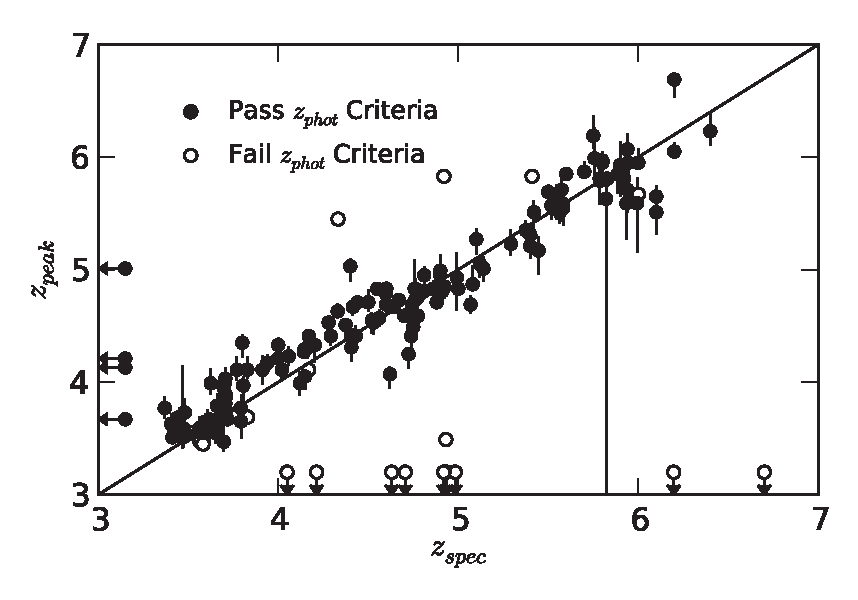
\includegraphics[width=84mm]{plots/fig1.eps}
\caption{Comparison between spectroscopic and photometric redshift for the galaxies in our sample with available spectroscopy and spectroscopic redshift quality of `Good" or better. Filled circles show sources which pass our selection criteria (including interlopers), empty circles show spectroscopically confirmed high-redshift sources which do not pass the selection criteria. The photometric redshift shown is the peak of the probability distribution ($\chi^2$ minimum) with 1-$\sigma$ lower and upper limits.}
\label{fig:specz}
\end{figure}

Figure~\ref{fig:specz} compares the available spectroscopic redshifts for the galaxies in our sample with the corresponding best-fit photometric redshift (minimum $\chi^2$) as found by EAZY. In total, there are 151 spectroscopic redshift matches for galaxies which pass our selection criteria and are therefore included in our samples. In addition, there are a further 21 galaxies with spectroscopic redshifts of $z > 3.5$ which pass the signal to noise, AGN criteria but do not pass the photometric redshift criteria. Of these 21 galaxies, 12 are correctly identified as high redshift galaxies but are excluded due to poor fits (11) or have a redshift very close to the $z = 3.5$ limit but photometric scatter pushes the photometric redshift to below the criteria (1). The remaining 9 spectroscopically confirmed high-redshift sources have best-fit photometric redshifts of $z_{peak} < 3$. The simulations undertaken to correct for selection completeness are outlined in Section~\ref{sec:completeness}.

For the matched galaxies which pass our selection criteria, we find that our redshift accuracy is very good, with a scatter of just $\sigma_{z,O} = rms(\Delta z /1+z_{\text{spec}}) = 0.037$ when outliers are excluded, where $\Delta z =  (z_{\text{spec}}-z_{\text{phot}})$ \citep{Dahlen:2013eu}. We define outliers as $\left | \Delta z \right |/(1+z_{\text{spec}}) > 0.15$, and find an outlier fraction of 2.65\% (4 galaxies). This compares with \citet{2012ApJ...756..164F} who find a scatter of $\sigma_{z}/(1+z) = 0.044$  at $z > 3$ after excluding outliers (defined more strictly as $\left | \Delta z \right | > 0.5$) in the same CANDELS field. We also find that there is very little bias in our photometric redshifts, with $median(\Delta z) = -0.04$. Of the 4 galaxies classed as outliers, all lie at redshifts of $z < 3$ and are low-redshift interlopers which our selection criteria have not been able to exclude.

\citet{Dahlen:2013eu} have recently shown that by combining the results from multiple photometric redshift codes, the scatter and outlier fraction in photometric redshifts can be significantly reduced compared to the results of any single code. For the same set of 151 spectroscopic redshift sources, the photometric redshifts produced through the Bayesian combination outlined in \citet{Dahlen:2013eu} have $\sigma_{z,O} = 0.033$ with an outlier fraction of 3.98\% and $median(\Delta z) = 0.01$. 

Although utilising the photometric redshifts for the CANDELS GOODS-S field produced by this method would result in a small gain in photometric accuracy, we would no longer be able to reproduce the full selection method when running simulations. Given this small improvement, we are confident that the use of photometric redshifts produced by a single code will not adversely affect the overall accuracy of the results.

The matched spectroscopic redshifts are from the following surveys: \citet{LeFvre:2004ge,Stanway:2004gu,Vanzella:2008hp,Hathi:2008ca,Popesso:2009ht,Wuyts:2009gv,Rhoads:2009eb,Vanzella:2009ez,Balestra:2010bt,Kurk:2012ej}. The high-redshift spectroscopic sources within these surveys all derive from initial target selections of predominantly bright Lyman Break galaxy candidates. The measured photometric redshift accuracies are therefore likely biased to a better scatter than the full high-redshift galaxy population. However, examining the redshift accuracy of the mock galaxy catalog used for our selection comparisons in Appendix~\ref{app:selection}, we find that the photometric redshift accuracy remains good down to the lowest masses probed in this survey for galaxies which pass our criteria. For example, for galaxies of $\text{M}_{*} \approx 10^{8.5} \text{M}_{\odot}$, we find a scatter excluding outliers of $\sigma_{z,O} = 0.053$ and $median(\Delta z) = 0.025$ before any $P(z)$ criteria are applied.

To investigate how the SMF evolves from z = 4-7, we then constructed four redshift samples in bins across this redshift range: $z \sim 4 ~(3.5 \leq z < 4.5)$, $z \sim 5~ (4.5 \leq z < 5.5)$, $z \sim 6~(5.5 \leq z < 6.5)$ and $z \sim 7 ~(6.5 \leq z < 7.5)$.

\subsection{Monte Carlo Samples}\label{sec:MC}
Although we find that our photometric redshifts do well when compared with the matched spectroscopic redshifts, the group of outliers are indicative of the difficulties that exist in correctly distinguishing between the Lyman break of high-redshift galaxies at $z > 3$ and strong Balmer break galaxies at more moderate redshifts $z \approx 0.5-2.5$ in low S/N data. \citet{2012ApJ...748..122P,Pirzkal:2013ug} have shown that it is very difficult to categorically classify sources as high-redshift galaxies and not low-redshift interlopers using photo-z's or S/N criteria on the dropout bands.

Previous work using photometric redshifts has dealt with this problem by making use of the full redshift PDF when calculating luminosity functions \citep{2005ApJ...631..126D,2009MNRAS.395.2196M,McLure:2013hh}, thereby incorporating the uncertainty in the analysis. Due to the nature of the SED fitting code used for this work (described in Section~\ref{sec:masses}), the computational effort required to fit the mass at each redshift in order to integrate over the full PDF becomes impractical. As such, we chose to account for these problems in a different manner whilst still dealing with them in a straight-forward way. 

Rather than using only the best-fit redshift from our photometric analysis when selecting our sample, we instead draw the redshift for each galaxy randomly from its full PDF before placing it in the appropriate redshift sample. Where secure spectroscopic redshifts are available, we fix the redshift to that value for all samples (known interlopers are therefore excluded in all samples). This process was repeated 500 times to produce a set of samples to which we then apply the rest of the analysis described in the paper separately. We then average over the results from each sample, using the mean of this full set as our `true' value along with the 1-$\sigma$ upper and lower limits around this mean. 

\begin{table}
\caption{Average sample size and variance for each redshift bin for the 500 Monte Carlo samples generated, see text for details.}
\label{tab:samplesizes}
\begin{tabular}{@{}ccc}
\hline
 Redshift Bin & Mean Sample Size & Variance on sample size  \\
  \hline
 4 & 1235 & 180 \\
 5 & 416 & 63 \\
 6 & 169 & 25 \\
 7 & 42 & 9 \\
 \hline
\end{tabular}
\end{table}

The resulting sample sizes for each redshift bin are shown in Table~\ref{tab:samplesizes}. The varying samples account for both scattering between redshift bins for objects at the boundaries as well as objects moved out of the sample into secondary low-redshift solutions. The effect of this scattering into and out of the samples can be seen when comparing the combined mean samples sizes (1862) to our full high-redshift sample of 2263.

\begin{figure*}
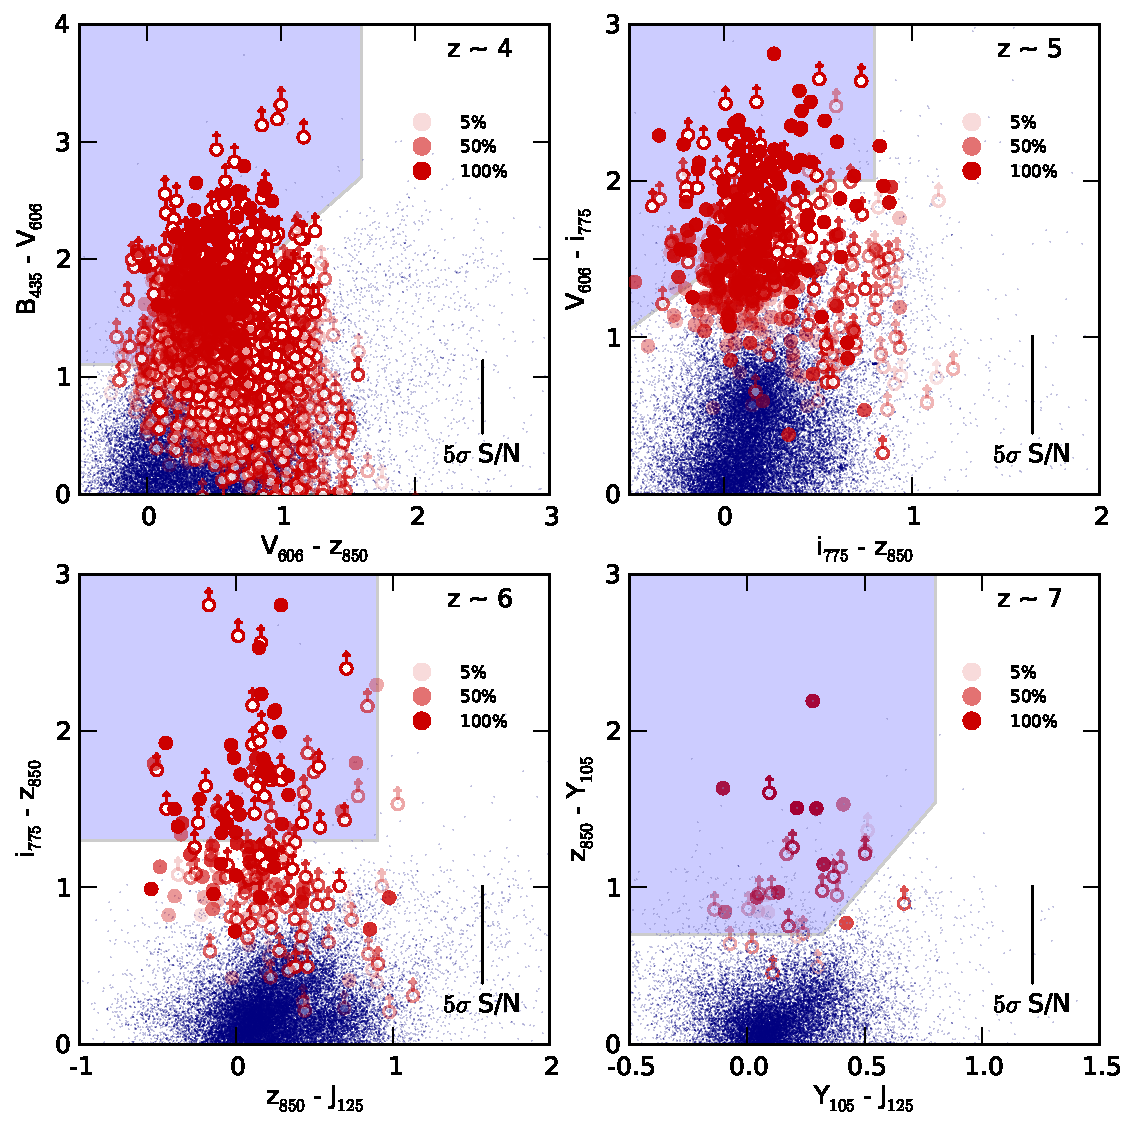
\includegraphics[width=140mm]{plots/fig2.eps}
\caption{The colours of our photometric redshift selected samples in relation to the two-colour cuts typically used to select Lyman break galaxies. Non-detections in a filter are converted to 2-$\sigma$ upper limits when calculating the colours. The shaded blue regions show the region in colour space used to select dropout galaxies in that redshift bin as described in  \citet{2007ApJ...670..928B} and \citet{2012ApJ...754...83B}. The blue points show the colours for the full GOODS-S photometric catalog from which we select our high redshift samples. Red symbols represent galaxies selected in our sample by our selection criteria, where the transparency of the symbols is determined by the number of Monte Carlo samples in which it is selected i.e. the fainter the symbol, the smaller the fraction of MC samples that galaxy is selected in. The legend in each plot illustrates this transparency for galaxies selected in 5, 50 and $100\%$ of Monte Carlo samples. Colours which make use of 2-$\sigma$ upper limits are plotted with open circles, while objects with 2-$\sigma$ detections or better in all bands are plotted with filled circles. Example error bars corresponding to 5-$\sigma$ detections (for both filters in a given colour) are shown for each of the corresponding drop-out colours.}
\label{fig:colours}
\end{figure*}

The strength of using photometric redshifts for sample selection over colour cuts (especially when redshifts would still need to be calculated for a colour-cut sample in order to do SED fitting) is that the method can automatically make use of all available photometry. This is important because although photometric redshifts are still fitting primarily to the characteristic break at Lyman-$\alpha$ targeted by the colour selections, the filters long-ward of the break are useful in excluding low-redshift interlopers \citep{2011MNRAS.418.2074M}. Additionally, the large errors in colour possible due to low signal to noise and possible non-detections in the filter just short of the Lyman break means that likely high-redshift candidates can be scattered well outside the selection region when using colour cuts. 

Figure~\ref{fig:colours} shows the positions of our galaxy samples on the colour-colour planes commonly used to select dropout samples. It is obvious that many of the galaxies selected with photometric redshifts lie outside the selection regions (as taken from \citeauthor{2007ApJ...670..928B}~\citeyear{2007ApJ...670..928B}), especially those galaxies where colours must be calculated using an upper limit. The agreement (or lack of) between dropout selections and photometric redshifts has also been investigated for GOODS-S specifically by \citet{2010ApJ...724..425D}.

To test whether the discrepancy between the observed colours and those required for Lyman break selection can be explained solely by photometric scatter, we performed a range of tests on a mock catalog generated from the semi-analytic models described in \citet{Somerville:2008ed} and \citet{Somerville:2012cq}. Full details of these tests are outlined in Appendix~\ref{app:selection}, however our main finding is that the observed colours can be reproduced from intrinsic Lyman break-like colours and scattering proportional to the observed photometric errors. 

\section{Selection method comparison}\label{app:selection}
Traditionally, (star-forming) galaxies at high-redshift have been selected using the Lyman break technique, whereby galaxies are selected based on the observed colours across the redshifted Lyman break in their spectra.

When the observed colours of our photometric redshift selected galaxies are plotted in the same way, the selected galaxies span a range of colours far wider than those encompassed by the Lyman break galaxy (LBG) selection criteria. Many of the galaxies have colours which would place them in the locus spanned by low-redshift galaxies, according to the Lyman break criteria. This has been observed before by \citet{2010ApJ...724..425D}, who find a similar range of colours for galaxies with photometric redshifts at $z \sim 4$ and 5.

This raises the question as to whether this discrepancy is solely due to photometric scatter in the relevant colours, if they have stellar populations different from those expected for the Lyman break criteria, or if in fact those galaxies outside the selection criteria are low-redshift interlopers or catastrophic failures in the photometric redshift estimation.

To answer these questions, we have taken a sample of mock galaxies from the CANDELS semi-analytic models of \citet{Somerville:2008ed} and \citet{Somerville:2012cq} across all redshifts. From the full SAM catalog of galaxies from $z = 0$ to $z > 8$, we have included all galaxies at $z > 3$ and a randomly selected sample of a quarter of the galaxies at $z = 3$ and below (subsequent calculations of the interloper fraction fully correct for this reduced number density at $z < 3$). The resulting sample of $\sim 260,000$ galaxies consists of approximately equal numbers of high-redshift galaxies and a fully representative sample of low-redshift galaxies across their corresponding luminosity and colour distributions. For full details of the mock galaxy properties as a function of redshift we refer the reader to \citet{Somerville:2008ed} and \citet{Lu:2013ui}.

We then assign photometric errors to the intrinsic fluxes in each band based on the observed errors in the original catalog and then perturb the flux by those errors. The resulting colours should then indicate the effects of photometric scattering on the intrinsic colours. We have assumed the errors are gaussian (the fluxes are perturbed by a value drawn from a gaussian where $\sigma =$ Flux Error) and have applied the errors based on the measured flux errors of objects with equivalent fluxes in the UDF, DEEP and WIDE regions. 

To further illustrate this process we also select an example galaxy from our mocks which we can follow through the individual steps. The photometric properties of the galaxy and the corresponding photometric errors are outlined in Table~\ref{tab:eg_photom}. The galaxy has a redshift of $z = 5.01$, a stellar mass of $\approx 8 \times 10^{8} \text{M}_{\odot}$ and a UV-continuum slope of $\beta = -2.1$.
 
\begin{table*}
    \centering
    \label{tab:eg_photom}
    \caption{Intrinsic magnitudes, fluxes and typical observation errors for the example galaxy and the CANDELS GOODS South region. The first row outlines the true intrinsic fluxes $F_{true}$ in the key filters at $z\sim5$. In the second row we show the measured 5-$\sigma$ limiting magnitudes (or fluxes) for the DEEP region estimated in \citet{Guo:2013ig} for the photometry used in this paper. The third row shows the average and standard deviation flux error for objects in the photometric catalog \citep{Guo:2013ig} with fluxes within 0.1 dex of the intrinsic flux for our example galaxy (i.e. the distribution from which our assigned photometric error is drawn). The final row shows the 'observed' fluxes ($F_{obs}$) for our example galaxy after assigning a flux error $\sigma_{F}$ and perturbing the intrinsic flux by a value drawn from a gaussian with width $\sigma = \sigma_{F}$.}
    \begin{tabular}{lcccccccc}
    \hline
    ~                      & \multicolumn{2}{c}{$V_{606}$} & \multicolumn{2}{c}{$i_{775}$} & \multicolumn{2}{c}{$z_{850}$} & \multicolumn{2}{c}{$H_{160}$} \\ \hline
    ~                      & AB        & $\mu Jy$ & AB & $\mu Jy$ & AB & $\mu Jy$ & AB   & $\mu Jy$ \\ \hline
    Intrinsic Flux - $F_{true}$           & 29.35         & 0.0066   & 27.14  & 0.0506  & 26.83  & 0.0673 & 26.91 &  0.0625  \\
    DEEP 5-$\sigma$ limit   & 29.35        & 0.0066   & 28.55  & 0.0138  & 28.55  & 0.0138 & 27.36 &  0.0413   \\
    Mean Error $\pm 1$ SD  & -         & $0.0054\pm0.0028$    & -  & $0.0111 \pm  0.0057$  &   & $0.0145 \pm 0.0113$   &   -   & $0.0099 \pm 0.0074$ \\ 
%    Assigned Error $F_{err}       & ~         & ~        & ~  & ~         & ~  & ~         & ~         & ~        \\ 
    'Observed' Flux - $F_{obs}$  & $>27.82$     & $0.009 \pm 0.009$  & 27.07  & $0.054\pm0.010$  & 26.85 & $0.066\pm0.013$   & 27.01        & $0.057 \pm 0.006$   \\
% When using 1-sigma colours: V = 28.981 +/- 1.04 
    \hline
    \end{tabular}
\end{table*}
 
\begin{figure}
\centering
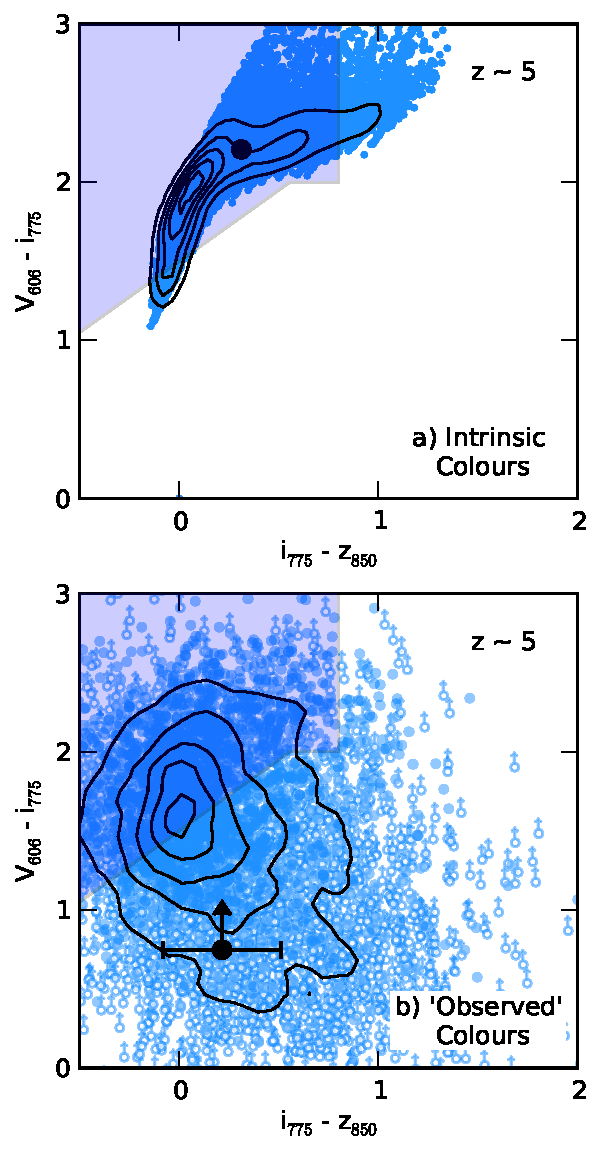
\includegraphics[width=80mm]{plots/figA1.eps}
\caption{a) Intrinsic colours of galaxies at $4.5 < z < 5.5$ from the CANDELS semi-analytic mock catalog. Also shown are contours representing the density of points, with the innermost contour corresponding to five times the density of the outermost contour. The larger black point shows the intrinsic colour of the galaxy from the example outlined in the text. b) Observed colours of galaxies at $4.5 < z < 5.5$ from SAM mock sample after the photometry has been perturbed by flux errors proportional to the observed flux errors in the CANDELS DEEP region of observed photometry. Open circles represent colours constructed from 2-$\sigma$ upper limits. As in a), the innermost contour corresponds to five times the density of points of the outermost contour.}
\label{fig:mock_col}
\end{figure}

The intrinsic colours of the mock galaxies at $z \sim 5$ ($4.5 \leq z < 5.5$) are shown in Figure~\ref{fig:mock_col}. It is clear that the colours spanned by the galaxies lie well within the Lyman break selection criteria of \citet{2007ApJ...670..928B}, with only a small fraction of galaxies redder than the criteria in the colour above the break or bluer across the Lyman break. Our input population therefore closely matches the colours for which the colour-colour criteria have been designed. The same is true across all redshift bins. 

The lower panel of Figure~\ref{fig:mock_col} shows the colours of our mock galaxy catalog after being perturbed by errors drawn from the CANDELS DEEP region. Only galaxies with $S/N(H_{160}) > 5$ are shown, matching the selection criteria for our high-redshift samples, resulting in a sample of 5673 galaxies with $4.5 < z_{\text{true}} < 5.5$. As for our observed objects in Figure~\ref{fig:colours}, 2-$\sigma$ upper-limits are used to derive magnitudes for non-detections ($S/N < 2$) and objects with negative fluxes.  

It is immediately clear that photometric scatter pushes the colour spanning the Lyman break to values much lower in $V_{606} - i_{775}$ than the range covered by the selection criteria. However, the main locus of galaxies still resides either within or within the typical error of the Lyman break selection region. In addition, the majority of mock galaxies with `observed' $V_{606} - i_{775} < 1$ are those with a non-detection in $V_{606}$ and hence represent a lower limit. The same effect occurs across all regions, with the lower photometric errors in deeper GOODS South region resulting only in a fainter magnitude for an equivalent signal to noise in the optical bands. 

The systematic shift towards lower values of $V_{606} - i_{775}$ once photometric scatter is included can be explained by the relative signal-to-noise ratios in the filters above and below the Lyman break. Given the depth of each filter (see Table~\ref{tab:eg_photom}), objects with relatively faint apparent magnitudes above the break and intrinsic colours $> 1-2$ will always have a significantly lower signal-to-noise in the filter below the break. In this scenario, $V_{606}$ fluxes which are scattered to higher values will result in a brighter more robust magnitude. Conversely, objects which are scattered to fainter magnitudes are more likely to result in non-detections, requiring the use of upper limits which will push the observed colours down.

These simulations show that high-redshift galaxies can exhibit colours across the Lyman break well outside the traditional selection criteria. However, it is also important to show that the galaxies selected by photometric redshift with colours outside the colour criteria are indeed these high-redshift galaxies rather than lower redshift galaxies in the same colour space.

\begin{figure}
\centering
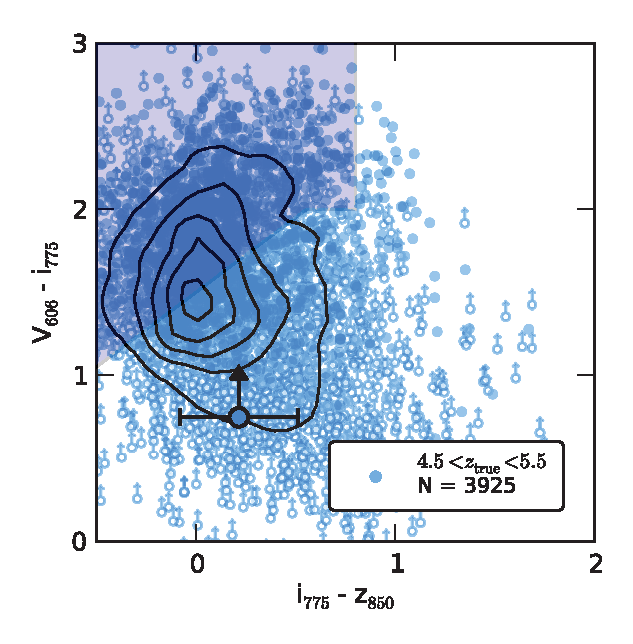
\includegraphics[width=80mm]{plots/figA2a.eps}
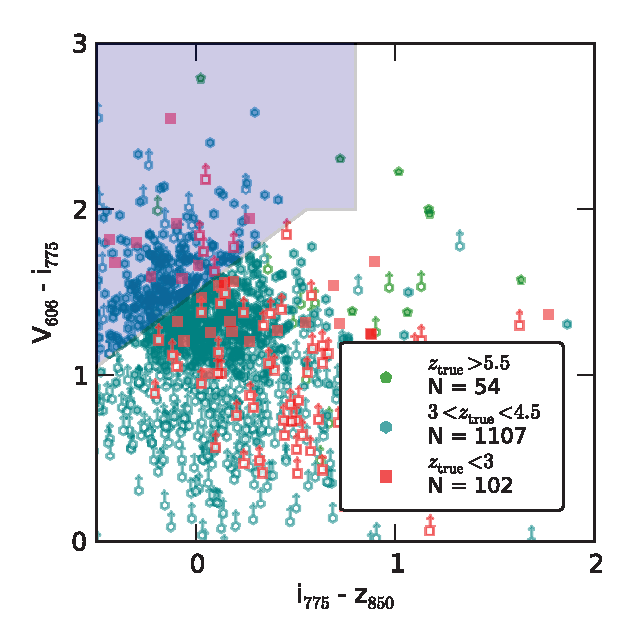
\includegraphics[width=80mm]{plots/figA2b.eps}
\caption{\emph{Top:} Observed colours of galaxies from the SAM mock sample which pass our photometric redshift selection criteria, have best-fitting photometric redshifts in the range $4.5 < z_{\text{phot}} < 5.5$ and have true redshifts in the range $4.5 < z_{\text{true}} < 5.5$. As in Figure~\ref{fig:mock_col}, the innermost contour corresponds to five times the density of points of the outermost contour. Open circles with arrows represent colours constructed from 2-$\sigma$ upper-limits. The separately marked large blue circle corresponds to the the example galaxy which is correctly estimated to be $z \sim 5$. \emph{Bottom:} Observed colours of galaxies from the SAM mock sample which pass our photometric redshift selection criteria and have best-fitting photometric redshifts in the range $4.5 < z_{\text{phot}} < 5.5$ but have true redshifts outside of the desired redshift bin. As in the top panel, open symbols with arrows represent colours constructed from 2-$\sigma$ upper-limits. In both panels, N is the number of galaxies in the corresponding sample. As outlined in the text, the number of $z_{\text{true}} < 3$ galaxies shown represents a quarter of those expected in a fully representative sample. Using the best-fitting photometric redshift and our selection criteria, the low-redshift interloper fraction for this sample $= (102 \times 4) / (54 + (102 \times 4) + 1107 + 3925) = 0.07$. This low-redshift interloper fraction is reduced to $\approx 0.06$ when we generate our Monte Carlo samples.}
\label{fig:mock_col_photz}
\end{figure}

To address this, we next calculate photometric redshifts for the SAM mock galaxy sample incorporating the photometric errors using the same method as described in Section 2 and apply our sample selection criteria. By applying additional cuts based on the full $P(z)$ distribution, the number of interlopers can be reduced at the expense of excluding some real sources.  How strict the selection criteria are is a balance between minimising the contamination from interlopers and scatter at the bin edges and maximising the number of real high-redshift galaxies in the sample. In Figure~\ref{fig:mock_col_photz} we show the colours of galaxies which pass our high-redshift selection criteria. The top panel of Figure~\ref{fig:mock_col_photz} shows those galaxies with $4.5 < z_{\text{true}} < 5.5$, these galaxies span the full range of colours traced by the error perturbed colours of input high-redshift galaxies shown in the previous plots. In the case of the Table~\ref{tab:eg_photom} example galaxy, the best-fitting photometric redshift is $z = 5.0^{+0.2}_{-0.5}, 5.2\pm0.1$ and $4.86^{+0.27}_{-0.15}$ for the DEEP, UDF and WIDE errors respectively. 

In the bottom panel of Figure~\ref{fig:mock_col_photz}, we show the selected galaxies which have true redshifts outside of the desired redshift range. At $z\sim 5$, the majority of low-redshift ($z < 3$) interlopers which are selected to be $z\sim5$ by the photometric redshift selection exhibit colours which lie outside of the Lyman break colour criteria. The fraction of low-redshift interlopers is very small compared to the number of 'real' high-redshift galaxies in this colour space. However, as redshift increases, the fraction of low-redshift interlopers increases such that at $z \sim 7$ based on the best-fitting $z_{peak}$ alone, the fraction of outliers equals $\sim 0.60$, 0.51 and 0.72 for DEEP, UDF and WIDE respectively. Clearly, basing high-redshift samples on the best-fitting photometric redshift alone would produce highly biased samples. Further $S/N$ or photometric criteria such as those used in this work are clearly required to produce a reliable sample.

Applying the selection criteria and generating Monte Carlo samples as outlined in Section~\ref{sec:sample}, the low-redshift interloper fractions for our mock samples are reduced to an estimated 0.008, 0.06, 0.15 and 0.22 for $z \sim 4$, 5, 6 and 7 respectively. This was estimated by combining the fractions calculated for each field (assuming the ERS region to have interloper fractions comparable to the DEEP region) proportional to the number of high-redshift galaxies selected from each region of the field. 

The lower panel of Figure~\ref{fig:mock_col_photz} also highlights the importance of fully incorporating the photometric redshift errors when creating high-redshift galaxy samples. Approximately 20\% of the galaxies selected as $z\sim5$ have true redshifts below the desired range. However upon closer inspection, we find that the median true redshift for the $3 < z_{\text{true}} < 4.5$ points (turquoise hexagons) is 4.4 whilst the median best-fitting photometric redshift for the same sample is $4.6$ with average 1-$\sigma$ errors of $^{+0.18}_{-0.35}$.

By making use of the full $P(z)$ distribution estimated by the photometric redshift code as we do in this work (see Section~\ref{sec:MC}), galaxies with $P(z)$ which span the redshift boundaries will be scattered between and contribute to both adjacent redshifts bins between different MC samples (or scattered out of the sample e.g. $z < 3.5$ or $z > 7.5$). Throughout this work, the errors resulting from this photometric redshift uncertainty are incorporated in the analysis and errors presented.

\begin{figure}
\centering
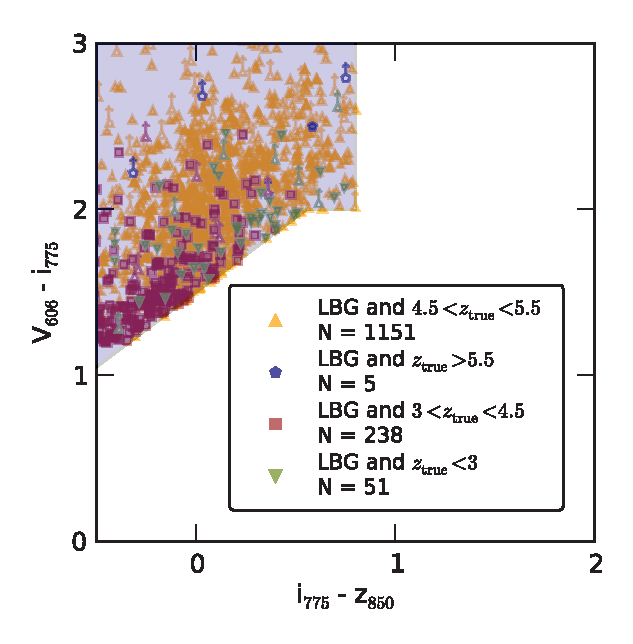
\includegraphics[width=80mm]{plots/figA3a.eps}
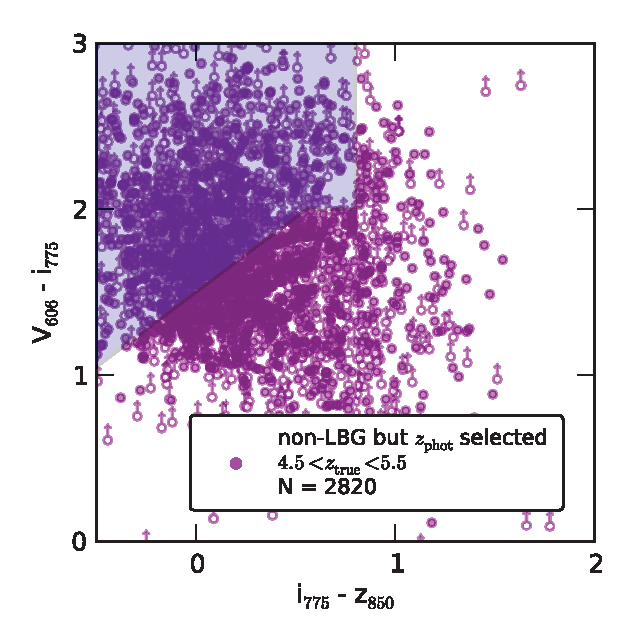
\includegraphics[width=80mm]{plots/figA3b.eps}
\caption{\emph{Top:} Observed colours of galaxies from the SAM mock sample which pass the Lyman break selection criteria outlined in the text, separated into bins of intrinsic redshifts. In contrast to previous plots and in keeping with common LBG selection techniques, when calculating colours the measured magnitude is used down to a $S/N = 1$ and the 1-$\sigma$ upper limit is used below this. The same is true for colours plotted in the bottom panel. As outlined in the text, the number of $z_{\text{true}} < 3$ galaxies shown represents a quarter of those expected in a fully representative sample. The low-redshift interloper fraction for this sample $= (4*51) / (5 + (51 \times 4) + 238 + 1151) = 0.13$. \emph{Bottom:} Observed colours of galaxies from the SAM mock sample with $4.5 < z_{\text{true}} < 5.5$ which fail the Lyman break selection criteria outlined in the text but are correctly selected as $z\sim5$ galaxies by the photometric redshift selection used in this work.}
\label{fig:mock_col_LBG}
\end{figure}

To compare the low-redshift interloper fractions and the robustness of our photometric redshift selection, we also run the SAM mock catalog through a Lyman break selection process. Our Lyman break selection criteria are based on the $V_{606}$-dropout criteria of \citet{2012ApJ...754...83B} and we exclude sources with $S/N > 2$ in any of the bands blueward of the dropout bands ($U_{\text{CTIO}}$, $U_{\text{VIMOS}}$ and $B_{435}$). We also require $S/N(i_{775}) > 5.5$, comparable with other Lyman break selections at this redshift, e.g. \citet{Giavalisco:2004et} and \citet{2006AJ....132.1729B}. However we note that by choosing a stricter optical $S/N$ requirement, the purity of the sample can always be improved at the expense of total sample size. For consistency with other LBG selections, when making the colour cuts, we use the observed magnitudes for detections above 1-$\sigma$ and the 1-$\sigma$ upper limit below this.

We caution that since the mock photometric catalog in this section is designed to replicate the $H_{160}$ selection of the observational data used in this paper, the detection criteria for our Lyman break sample will differ from those in the literature based solely on the optical (e.g. \citeauthor{2007ApJ...670..928B}~\citeyear{2007ApJ...670..928B}). Therefore, the selection efficiencies and low-redshift interloper fractions calculated here represent only the Lyman break technique as applied to the CANDELS data in this paper specifically. As such, we do not make any claims regarding the low-redshift interloper fraction of Lyman break selection elsewhere in the literature.

In the upper panel of Figure~\ref{fig:mock_col_LBG}, we show the colour distribution and sample sizes for our LBG sample. For this sample, we find a low-redshift interloper fraction comparable to that of the photometric redshift selection. In the lower panel of Figure~\ref{fig:mock_col_LBG}, we show galaxies which have true redshifts in the range $4.5 < z_{\text{true}} < 5.5$ and do not satisfy all of the LBG criteria but do pass the photometric redshift selection criteria. Although many of these galaxies have colours outside the LBG colour criteria, photometric redshifts are also able to select galaxies which fail the non-detection or optical $S/N$ criteria. In Figure~\ref{fig:mock_z_hist}, we also compare the intrinsic redshift distribution of the two selection methods. Both the low-redshift contaminants and scatter at bin extremities are clearly visible for both samples.

\begin{figure}
\centering
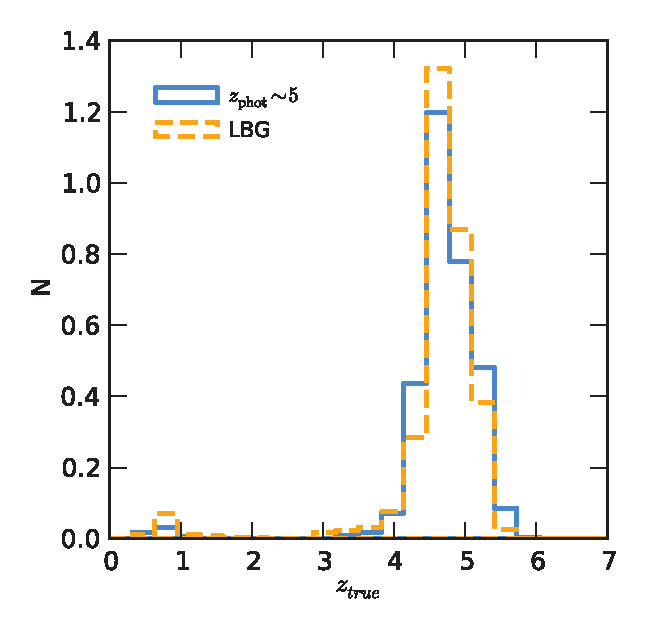
\includegraphics[width=80mm]{plots/figA4.eps}
\caption{Normalised number densities as a function of true redshift for the photometric redshift and Lyman break galaxy samples generated for our SAM mock galaxy catalog.}
\label{fig:mock_z_hist}
\end{figure}


\begin{figure}
\centering
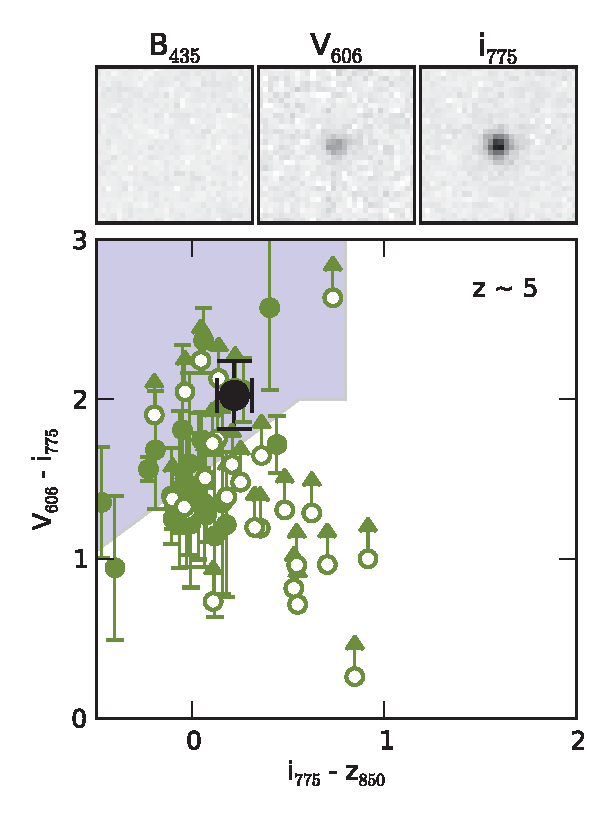
\includegraphics[width=80mm]{plots/figA5.eps}
\caption{\emph{Top panels}: $1.8 \times 1.8$ arcsec$^2$ postage-stamp images of the median stacked faint sources in the $B_{435}$, $V_{606}$ and $i_{775}$ filters. \emph{Main panel}: The observed colours of the individual faint sources are shown by the smaller green circles. Open circles represent sources where the $V_{606}$ has been calculated from the $2\sigma$ flux upper limit. The large black circle shows the measured colour for the stacked images.}
\label{fig:stack_colours}
\end{figure}

As a further step to demonstrate the difference in the observed Lyman break colours can be explained solely by photometric scatter, we examine the photometry for a median stack of the 50 candidate $z \sim 5$ galaxies in the CANDELS DEEP region with the lowest $S/N(H_{160})$. Stacking the photometry of a large enough number of sources should cancel out most of the photometric noise, with the resulting images closely reproducing the average intrinsic colours of the input galaxies. In Figure~\ref{fig:stack_colours}, we show the initial observed colours (or lower limits) for each of the faint $z\sim5$ candidates along with the observed colours of the stacked sources. Although the majority of the input galaxies have colours outside the Lyman break selection, the combined stack has a colour which places it more than 1-$\sigma$ inside the desired region and fully consistent with the expected $z \sim 5$ colours.

Also shown in Figure~\ref{fig:stack_colours} are the median stacked images in the 3 filters from below to above the Lyman break. Crucially, for any high-redshift candidate galaxy, the filters at wavelengths lower than the Lyman selection colours should contain zero flux due to the complete absorption by inter-galactic Hydrogen. The median stack in $B_{435}$ for our faint sample contains no trace of flux, with a 2-$\sigma$ upper limit of $29.48$ within a $0.6"$ diameter aperture.

While the tests presented in this appendix cannot account for objects with peculiar intrinsic colours (i.e. significantly different from those predicted by semi-analytic or synthetic stellar population models), they demonstrate that the observed colour distribution can be fully accounted for by the photometric scattering of the expected intrinsic colours. We also conclude that photometric redshift selection can be much less sensitive to photometric scatter than the Lyman break selection criteria for the same redshift range. Furthermore, that it is also able to correctly select high-redshift galaxies which are not identified by the traditional Lyman break selection techniques. In addition, the samples produced by both methods contain similar fractions of low-redshift galaxy contamination when criteria of comparable strictness are applied.


%% %% End of file...  %%
